\documentclass[11pt]{scrreprt}

\usepackage[T1]{fontenc}
\usepackage[utf8]{inputenc}
% \usepackage[ngerman]{babel}

\usepackage{graphicx}
\graphicspath{ {imgs/} {../evaluation/graphbrain_semsim/case_studies/plots/}}

\usepackage[backend=biber, style=alphabetic]{biblatex}
%\usepackage[backend=bibtex, style=authoryear-comp]{biblatex}
\newcommand{\citep}{\parencite}  % adds \citep alias for citing with parenthesis

\usepackage{amsmath}

\usepackage{parskip}
\usepackage{hyperref}
\usepackage{caption}
\usepackage{subcaption}


\usepackage{newfloat}
\DeclareFloatingEnvironment[
  listname = {List of Patterns} ,
  name = Pattern,
  placement = h,
  within = none
]{pattern}

%\let\textsf\undefined
%\newcommand{\textsf}[1]{\normalfont\sffamily #1}}}
%\newcommand{\textsfs}[1]{{\small{\normalfont\sffamily #1}}}
%\newcommand{\textsft}[1]{{\tiny{\normalfont\sffamily #1}}}

\addbibresource{MA.bib}

\usepackage{lipsum}  % produces dummy text
\begin{document}

% ========== Title page

\titlehead
{
\begin{tabular}{ll}
\begin{minipage}{0.5\textwidth}
	\textbf{Technische Universität Berlin} \\
	Fakultät IV: Elektrotechnik und Informatik \\
	Institut für Telekommunikationssysteme \\
	Fachgebiet Verteilte offene Systeme	
\end{minipage}
&
\begin{minipage}{0.5\textwidth}
	\raggedleft
	
\includegraphics[width=0.3\textwidth]{logos/tub_logo_bw.jpg}			
\end{minipage}

\end{tabular}
}

\subject{Masters Thesis in Computer Science}
\title{Extending Semantic Hypergraphs by neuronal semantic similarity matching to ???}
\author{Max Reinhard}

\date{\today}
\publishers{Supervised by Prof. Dr. Manfred Hauswirth \\
	Additional guidance by Prof. Dr. Camille Roth\thanks{Centre Marc Bloch (An-Institut der Humboldt-Universität zu Berlin)} \ 
	and Dr. Thilo Ernst\thanks{Fraunhofer-Institut für offene Kommunikationssysteme}}
	


\maketitle

% ========== Abstract
\begin{abstract}
\textbf{Abstract}
\lipsum[1-2]
\end{abstract}

% ========== TOC
\tableofcontents
\newpage

% ========== Body
% ==============================

% ========== 
\chapter{Introduction}
\begin{itemize}
	\item Context: The big problem
	\item Problem statement: The small problem
	\item Methodology / Strategy
	\item Structure
\end{itemize}

\textbf{Notes:}
\begin{itemize}
	\item Huge amounts of text, which can provide insight about stuff
	\item Automatic tools can provide assistance for humans to process all the text
	\item This generally means filtering the original text corpus or otherwise reducing amount of information the information that has to be processed by humans
	\item Filtering introduces a bias
	\item Especially for scientific purposes it is relevant to mitigate bias or at least understand what bias has been introduced (to make it transparent)
	\item Semantic Hypergraphs can be a valuable tool for that because...
\end{itemize}

A Semantic Hypergraph (SH) \citep{menezes_semantic_2021} is...



% ========== 
\chapter{Fundamentals and Related Work}
\section{Semantic Hypergraph}

\subsection{Notation}

Square bracket notation 


\section{Text Similarity Measures}

tf-idf, etc.?


\section{Semantic Similarity}


\section{Embedding-based similarity}

\subsection{Embedding types}

\subsubsection{Fixed word embeddings}

\subsubsection{Contextual embeddings}

\subsubsection{Sentence embeddings}

\subsection{Embedding distance measures}




% ========== 
\chapter{Solution Approach}

Combining Semantic Hypergraphs with neural embeddings

\section{\texttt{semsim} Functional Pattern}

\subsection{Pattern-wise Similarity Threshold}


\section{Fixed word-vector based}

\subsection{Single Word}

\subsection{Multi Word}
\label{sec:semsim-multi-word}


% ========== 
\chapter{Implementation}

\section{Integration into the SH Framework}
Realisation as functional pattern


\section{External Libraries and Models}
Word2Vec
Gensim






\section{SH Notation}
Bracket notation for multi-word Semsim



% ========== 
\chapter{Results and Evaluation}
%\section{Qualitative Results}
\section{Case Study: Conflicts}
This case study follows the approach presented in \cite[p.~22]{menezes_semantic_2021} where expressions of conflict are extracted from a SH constructed from a corpus of news titles that were shared on the social media platform \textit{Reddit}. Specifically all titles shared between January 1st, 2013 and August 1st, 2017 on \textit{r/worldnews}\footnote{\url{http://reddit.com/r/worldnews}}, which is described as: “A place for major news from around the world, excluding US-internal news.”

Pattern \ref{pat:conflict} is used to extract conflicts between two parties, where the \textsf{SOURCE} shows some form of aggression against the \textsf{TARGET}, potentially regarding some \textsf{TOPIC}:

\begin{pattern}
  \normalfont\sffamily
  \centering
  ( PRED/P.{so,x} SOURCE/C TARGET/C [against,for,of,over]/T TOPIC/[RS] ) \(\wedge\)\\ ( lemma/J >PRED/P [accuse,arrest,clash,condemn,kill,slam,warn]/P )
  \caption{Conflict pattern}
  \label{pat:conflict}
\end{pattern}



To investigate whether it is possible to capture the abstract concept of a country using the multi-word \texttt{semsim} pattern introduced in \ref{sec:semsim-multi-word}, a list of the 20 most populous countries \citep{wiki:list_of_countries} is used:

\textit{China, USA, Indonesia, Pakistan, Nigeria, Brazil, Bangladesh, Russia, Mexico, Japan, Philippines, Ethiopia, Egypt, Vietnam, Congo, Iran, Turkey, Germany, France}

Pattern \ref{pat:conflict-countries} shows the resulting pattern for conflicts between countries.

\begin{pattern}
  \normalfont\sffamily
  \centering
  ( PRED/P.{so,x} SOURCE/C TARGET/C semsim [against,for,of,over]/T TOPIC/[RS] ) \(\wedge\) \\ 
  ( semsim/J >/PRED/P [accuse,arrest,clash,condemn,kill,slam,warn]/P ) \(\wedge\) \\
  ( semsim/J >SOURCE/C [china,usa,indonesia,pakistan,nigeria,brazil,bangladesh,russia, mexico,japan,philippines,ethiopia,egypt,vietnam,congo,iran,turkey,germany,france]/C ) \(\wedge\) \\
  ( semsim/J >TARGET/C [china,usa,indonesia,pakistan,nigeria,brazil,bangladesh,russia, mexico,japan,philippines,ethiopia,egypt,vietnam,congo,iran,turkey,germany,france]/C )
  \caption{Country conflict pattern}
  \label{pat:conflict-countries}
\end{pattern}


In \ref{fig:case-study-conflict-countries} the number of matches that result from using this pattern is plotted against the similarity threshold for the \texttt{semsim} pattern.


\begin{figure}
     \centering
     \begin{subfigure}[t]{0.9\textwidth}
         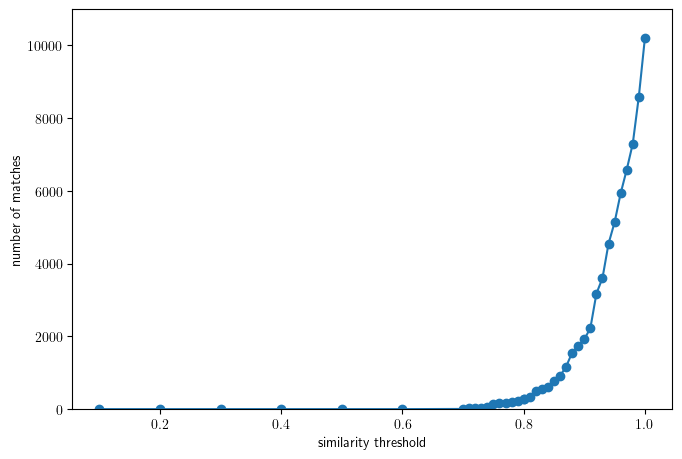
\includegraphics[width=\textwidth]{countries_20-most-popul_thresholds.png}
         \caption{Similarity threshold variation for all \textsf{semsim} patterns}
         \label{fig:countries_20-most-popul_thresholds}
     \end{subfigure}
     \begin{subfigure}[t]{\textwidth}
         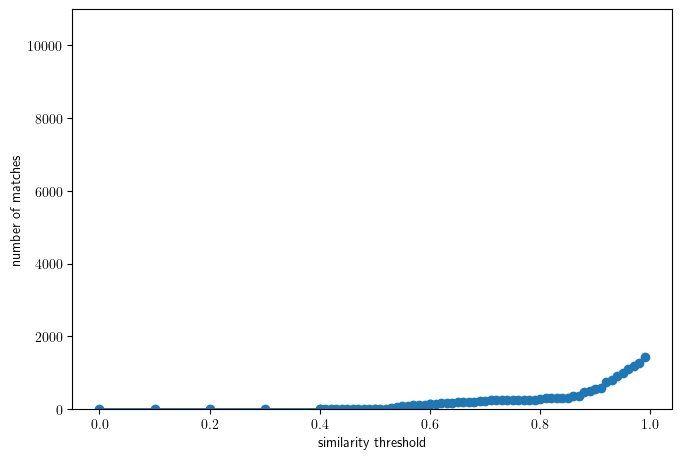
\includegraphics[width=\textwidth]{countries_20-most-popul_thresholds-countries.png}
         \caption{Similarity threshold variation only for \textsf{SOURCE} and \textsf{TARGET} (country) \texttt{semsim} patterns}
         \label{fig:countries_20-most-popul_thresholds-countries}
     \end{subfigure}
\caption{Number of matches for conflict pattern in relation to similarity threshold}
\label{fig:case-study-conflict-countries-1}   
\end{figure}

\begin{figure}
     \centering
     \begin{subfigure}[t]{0.9\textwidth}
         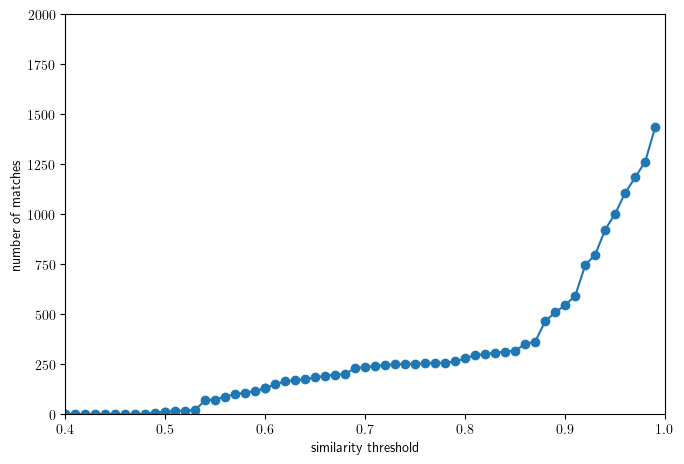
\includegraphics[width=\textwidth]{countries_20-most-popul_thresholds-countries_greater-0.4.png}
%         \caption{Similarity threshold variation only for \textsf{SOURCE} and \textsf{TARGET} (country) \texttt{semsim} patterns}
%         \label{fig:countries_20-most-popul_thresholds-countries-greater-0.4}
     \end{subfigure}
\caption{Number of matches for conflict pattern in relation to similarity threshold with threshold variation for \textsf{SOURCE} and \textsf{TARGET} (country) \texttt{semsim} patterns in the range \(0.4 >=\) threshold \(< 1.0\) (and y-axis limited to 2000 results)}
\label{fig:case-study-conflict-countries-2}   
\end{figure}


% ========== 
\chapter{Conclusion}




\printbibliography


\end{document}
